\documentclass[]{article}
\usepackage{lmodern}
\usepackage{amssymb,amsmath}
\usepackage{ifxetex,ifluatex}
\usepackage{fixltx2e} % provides \textsubscript
\ifnum 0\ifxetex 1\fi\ifluatex 1\fi=0 % if pdftex
  \usepackage[T1]{fontenc}
  \usepackage[utf8]{inputenc}
\else % if luatex or xelatex
  \ifxetex
    \usepackage{mathspec}
  \else
    \usepackage{fontspec}
  \fi
  \defaultfontfeatures{Ligatures=TeX,Scale=MatchLowercase}
\fi
% use upquote if available, for straight quotes in verbatim environments
\IfFileExists{upquote.sty}{\usepackage{upquote}}{}
% use microtype if available
\IfFileExists{microtype.sty}{%
\usepackage{microtype}
\UseMicrotypeSet[protrusion]{basicmath} % disable protrusion for tt fonts
}{}
\usepackage[margin=1in]{geometry}
\usepackage{hyperref}
\hypersetup{unicode=true,
            pdftitle={BI/Analytics Project},
            pdfborder={0 0 0},
            breaklinks=true}
\urlstyle{same}  % don't use monospace font for urls
\usepackage{color}
\usepackage{fancyvrb}
\newcommand{\VerbBar}{|}
\newcommand{\VERB}{\Verb[commandchars=\\\{\}]}
\DefineVerbatimEnvironment{Highlighting}{Verbatim}{commandchars=\\\{\}}
% Add ',fontsize=\small' for more characters per line
\usepackage{framed}
\definecolor{shadecolor}{RGB}{248,248,248}
\newenvironment{Shaded}{\begin{snugshade}}{\end{snugshade}}
\newcommand{\AlertTok}[1]{\textcolor[rgb]{0.94,0.16,0.16}{#1}}
\newcommand{\AnnotationTok}[1]{\textcolor[rgb]{0.56,0.35,0.01}{\textbf{\textit{#1}}}}
\newcommand{\AttributeTok}[1]{\textcolor[rgb]{0.77,0.63,0.00}{#1}}
\newcommand{\BaseNTok}[1]{\textcolor[rgb]{0.00,0.00,0.81}{#1}}
\newcommand{\BuiltInTok}[1]{#1}
\newcommand{\CharTok}[1]{\textcolor[rgb]{0.31,0.60,0.02}{#1}}
\newcommand{\CommentTok}[1]{\textcolor[rgb]{0.56,0.35,0.01}{\textit{#1}}}
\newcommand{\CommentVarTok}[1]{\textcolor[rgb]{0.56,0.35,0.01}{\textbf{\textit{#1}}}}
\newcommand{\ConstantTok}[1]{\textcolor[rgb]{0.00,0.00,0.00}{#1}}
\newcommand{\ControlFlowTok}[1]{\textcolor[rgb]{0.13,0.29,0.53}{\textbf{#1}}}
\newcommand{\DataTypeTok}[1]{\textcolor[rgb]{0.13,0.29,0.53}{#1}}
\newcommand{\DecValTok}[1]{\textcolor[rgb]{0.00,0.00,0.81}{#1}}
\newcommand{\DocumentationTok}[1]{\textcolor[rgb]{0.56,0.35,0.01}{\textbf{\textit{#1}}}}
\newcommand{\ErrorTok}[1]{\textcolor[rgb]{0.64,0.00,0.00}{\textbf{#1}}}
\newcommand{\ExtensionTok}[1]{#1}
\newcommand{\FloatTok}[1]{\textcolor[rgb]{0.00,0.00,0.81}{#1}}
\newcommand{\FunctionTok}[1]{\textcolor[rgb]{0.00,0.00,0.00}{#1}}
\newcommand{\ImportTok}[1]{#1}
\newcommand{\InformationTok}[1]{\textcolor[rgb]{0.56,0.35,0.01}{\textbf{\textit{#1}}}}
\newcommand{\KeywordTok}[1]{\textcolor[rgb]{0.13,0.29,0.53}{\textbf{#1}}}
\newcommand{\NormalTok}[1]{#1}
\newcommand{\OperatorTok}[1]{\textcolor[rgb]{0.81,0.36,0.00}{\textbf{#1}}}
\newcommand{\OtherTok}[1]{\textcolor[rgb]{0.56,0.35,0.01}{#1}}
\newcommand{\PreprocessorTok}[1]{\textcolor[rgb]{0.56,0.35,0.01}{\textit{#1}}}
\newcommand{\RegionMarkerTok}[1]{#1}
\newcommand{\SpecialCharTok}[1]{\textcolor[rgb]{0.00,0.00,0.00}{#1}}
\newcommand{\SpecialStringTok}[1]{\textcolor[rgb]{0.31,0.60,0.02}{#1}}
\newcommand{\StringTok}[1]{\textcolor[rgb]{0.31,0.60,0.02}{#1}}
\newcommand{\VariableTok}[1]{\textcolor[rgb]{0.00,0.00,0.00}{#1}}
\newcommand{\VerbatimStringTok}[1]{\textcolor[rgb]{0.31,0.60,0.02}{#1}}
\newcommand{\WarningTok}[1]{\textcolor[rgb]{0.56,0.35,0.01}{\textbf{\textit{#1}}}}
\usepackage{graphicx,grffile}
\makeatletter
\def\maxwidth{\ifdim\Gin@nat@width>\linewidth\linewidth\else\Gin@nat@width\fi}
\def\maxheight{\ifdim\Gin@nat@height>\textheight\textheight\else\Gin@nat@height\fi}
\makeatother
% Scale images if necessary, so that they will not overflow the page
% margins by default, and it is still possible to overwrite the defaults
% using explicit options in \includegraphics[width, height, ...]{}
\setkeys{Gin}{width=\maxwidth,height=\maxheight,keepaspectratio}
\IfFileExists{parskip.sty}{%
\usepackage{parskip}
}{% else
\setlength{\parindent}{0pt}
\setlength{\parskip}{6pt plus 2pt minus 1pt}
}
\setlength{\emergencystretch}{3em}  % prevent overfull lines
\providecommand{\tightlist}{%
  \setlength{\itemsep}{0pt}\setlength{\parskip}{0pt}}
\setcounter{secnumdepth}{0}
% Redefines (sub)paragraphs to behave more like sections
\ifx\paragraph\undefined\else
\let\oldparagraph\paragraph
\renewcommand{\paragraph}[1]{\oldparagraph{#1}\mbox{}}
\fi
\ifx\subparagraph\undefined\else
\let\oldsubparagraph\subparagraph
\renewcommand{\subparagraph}[1]{\oldsubparagraph{#1}\mbox{}}
\fi

%%% Use protect on footnotes to avoid problems with footnotes in titles
\let\rmarkdownfootnote\footnote%
\def\footnote{\protect\rmarkdownfootnote}

%%% Change title format to be more compact
\usepackage{titling}

% Create subtitle command for use in maketitle
\newcommand{\subtitle}[1]{
  \posttitle{
    \begin{center}\large#1\end{center}
    }
}

\setlength{\droptitle}{-2em}

  \title{BI/Analytics Project}
    \pretitle{\vspace{\droptitle}\centering\huge}
  \posttitle{\par}
    \author{}
    \preauthor{}\postauthor{}
    \date{}
    \predate{}\postdate{}
  

\begin{document}
\maketitle

\hypertarget{proposal}{%
\section{Proposal}\label{proposal}}

\hypertarget{deliverables}{%
\subsection{Deliverables}\label{deliverables}}

Week 7:

\begin{enumerate}
\def\labelenumi{\arabic{enumi}.}
\tightlist
\item
  Project Proposal

  \begin{itemize}
  \tightlist
  \item
    Together
  \end{itemize}
\item
  Design Document

  \begin{itemize}
  \tightlist
  \item
    Brenden
  \end{itemize}
\item
  Ensure installation of R is possible

  \begin{itemize}
  \tightlist
  \item
    McKay
  \end{itemize}
\item
  Risks

  \begin{itemize}
  \tightlist
  \item
    McKay
  \end{itemize}
\end{enumerate}

Week 8:

\begin{enumerate}
\def\labelenumi{\arabic{enumi}.}
\tightlist
\item
  two cleaning methods each

  \begin{itemize}
  \tightlist
  \item
    Filtering (NA's etc)

    \begin{itemize}
    \tightlist
    \item
      Brenden
    \end{itemize}
  \item
    Remove unnecessary columns

    \begin{itemize}
    \tightlist
    \item
      Brenden
    \end{itemize}
  \item
    Prepping secondary data for joins

    \begin{itemize}
    \tightlist
    \item
      McKay
    \end{itemize}
  \item
    Joins

    \begin{itemize}
    \tightlist
    \item
      McKay
    \end{itemize}
  \end{itemize}
\item
  1 profiling example each

  \begin{itemize}
  \tightlist
  \item
    Summary of deaths by year and month

    \begin{itemize}
    \tightlist
    \item
      Brenden
    \end{itemize}
  \item
    Summary of deaths by intent (homicide and suicide) and race

    \begin{itemize}
    \tightlist
    \item
      McKay
    \end{itemize}
  \end{itemize}
\item
  Installing R and RStudio
\item
  Learning basics of R
\item
  Pros and cons of cleaning and profiling in R

  \begin{itemize}
  \tightlist
  \item
    McKay
  \end{itemize}
\item
  List of things we learned
\end{enumerate}

Week 9:

\begin{enumerate}
\def\labelenumi{\arabic{enumi}.}
\tightlist
\item
  Write up pros and cons of R to Excel
\item
  2 patterns/visualizations/outliers each

  \begin{itemize}
  \tightlist
  \item
    Pairs plots

    \begin{itemize}
    \tightlist
    \item
      McKay
    \end{itemize}
  \item
    Boxplots

    \begin{itemize}
    \tightlist
    \item
      McKay
    \end{itemize}
  \item
    Bar-charts

    \begin{itemize}
    \tightlist
    \item
      Brenden
    \end{itemize}
  \item
    Outliers

    \begin{itemize}
    \tightlist
    \item
      Brenden
    \end{itemize}
  \end{itemize}
\item
  Pros and cons
\item
  List of things we learned
\end{enumerate}

Week 10:

\begin{enumerate}
\def\labelenumi{\arabic{enumi}.}
\tightlist
\item
  Pros and cons of R
\item
  List of things we learned
\item
  1 optimizing/forecasting/predicting model each

  \begin{itemize}
  \tightlist
  \item
    Trend prediction (shootings increasing by year in certain
    areas/races)

    \begin{itemize}
    \tightlist
    \item
      Brenden
    \end{itemize}
  \item
    Full regression analysis

    \begin{itemize}
    \tightlist
    \item
      McKay
    \end{itemize}
  \end{itemize}
\end{enumerate}

\hypertarget{description-of-problem}{%
\subsection{Description of Problem}\label{description-of-problem}}

With the hot topic of gun related crimes, we wanted to look at variables
that contribute to a person being killed by a gun. We were specifically
curious to look at school shootings, race fueled shootings, age, gender,
etc.

\hypertarget{dataset}{%
\subsection{Dataset}\label{dataset}}

\url{https://www.kaggle.com/hakabuk/gun-deaths-in-the-us}

\hypertarget{risks}{%
\subsection{Risks}\label{risks}}

\begin{enumerate}
\def\labelenumi{\arabic{enumi}.}
\tightlist
\item
  New team that has never worked together before

  \begin{itemize}
  \tightlist
  \item
    Team meetings at least once per week
  \end{itemize}
\item
  New software to one team member

  \begin{itemize}
  \tightlist
  \item
    McKay will help Brenden learn skills in R to complete this analysis
    while building his understanding of packages required for this
    analysis.
  \end{itemize}
\item
  Limitations of data on types of models possible

  \begin{itemize}
  \tightlist
  \item
    Searching for more supplementary data that may allow for other types
    of models
  \end{itemize}
\end{enumerate}

\hypertarget{ooda-design}{%
\subsection{OODA Design}\label{ooda-design}}

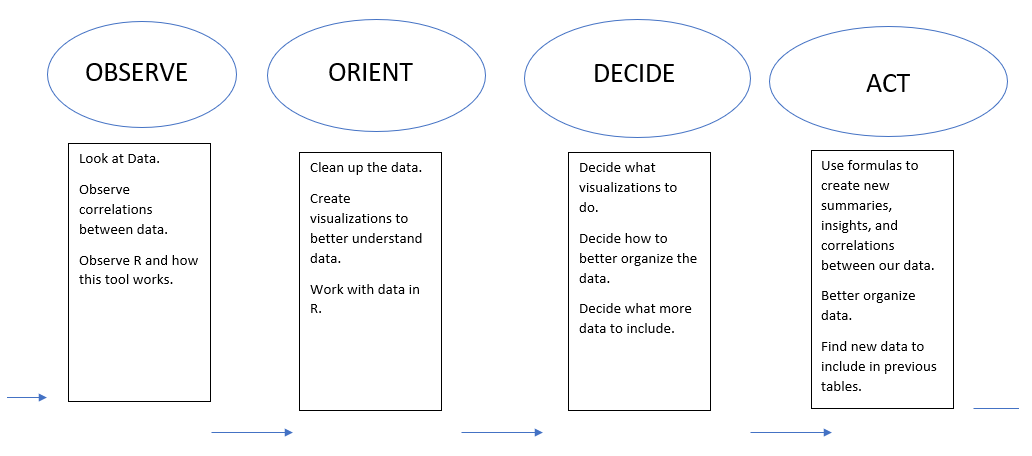
\includegraphics{../images/ooda.png}

\hypertarget{week-8}{%
\section{Week 8}\label{week-8}}

\hypertarget{work-done}{%
\subsection{Work Done}\label{work-done}}

\hypertarget{r-tutorials-brenden}{%
\subsubsection{R Tutorials (Brenden)}\label{r-tutorials-brenden}}

\hypertarget{regression-research-and-proscons-mckay}{%
\subsubsection{Regression Research and Pros/Cons
(McKay)}\label{regression-research-and-proscons-mckay}}

\begin{enumerate}
\def\labelenumi{\arabic{enumi}.}
\tightlist
\item
  Regression Research

  \begin{itemize}
  \tightlist
  \item
    We are probably going to need to run a chi-squared test as the y
    variable is likely going to be categorical and non-binary.
    \href{https://stats.idre.ucla.edu/other/mult-pkg/whatstat/}{click
    for source}
  \end{itemize}
\item
  Pros and Cons of R to Excel for cleaning and profiling

  \begin{itemize}
  \tightlist
  \item
    Pros

    \begin{itemize}
    \tightlist
    \item
      R code is modular and syntactically simple
    \item
      R is capable of handling larger data sets with far greater speed
    \item
      The user cannot physically touch the data and only touches states
      of the data, so there is not much room for accidentally deleting
      important things in the data.
    \item
      R has many more tools available to it than Excel.
    \item
      R is open source.
    \item
      Streamlined data merges.
    \end{itemize}
  \item
    Cons

    \begin{itemize}
    \tightlist
    \item
      Data cannot be directly modified in its tabular form. This is
      difficult for beginners.
    \item
      Pivot tables don't exist (although similar summaries of any kind
      can be created with relative ease).
    \item
      Excel is initially easier to use as most people have been exposed
      to similar Microsoft UI's since they were five or from its
      inception.
    \end{itemize}
  \end{itemize}
\end{enumerate}

\hypertarget{week-8-description-of-what-we-did}{%
\subsection{Week 8 Description of What We
Did:}\label{week-8-description-of-what-we-did}}

\hypertarget{edits-to-project-proposal}{%
\subsubsection{Edits to Project
Proposal:}\label{edits-to-project-proposal}}

\begin{enumerate}
\def\labelenumi{\arabic{enumi}.}
\tightlist
\item
  Changed cleaning methods and profiling to reflect what was needed
\item
  Edited pros/cons to be McKay's task (we still did some together)
\end{enumerate}

\hypertarget{methods}{%
\subsubsection{Methods:}\label{methods}}

We used the tidyverse package in R for reading in the data and cleaning
it. We used different methods included in the package. Below is our code
and outputs:

\begin{Shaded}
\begin{Highlighting}[]
\CommentTok{# libraries}
\KeywordTok{library}\NormalTok{(tidyverse)}
\end{Highlighting}
\end{Shaded}

\begin{verbatim}
## -- Attaching packages ------------------------------ tidyverse 1.2.1 --
\end{verbatim}

\begin{verbatim}
## √ ggplot2 3.0.0.9000     √ purrr   0.2.4     
## √ tibble  1.4.2          √ dplyr   0.7.4     
## √ tidyr   0.8.0          √ stringr 1.3.1     
## √ readr   1.1.1          √ forcats 0.3.0
\end{verbatim}

\begin{verbatim}
## -- Conflicts --------------------------------- tidyverse_conflicts() --
## x dplyr::filter() masks stats::filter()
## x dplyr::lag()    masks stats::lag()
\end{verbatim}

\begin{Shaded}
\begin{Highlighting}[]
\CommentTok{# Read in some data}
\NormalTok{guns <-}\StringTok{ }\KeywordTok{read_csv}\NormalTok{(}\StringTok{"../data/guns.csv"}\NormalTok{)}
\end{Highlighting}
\end{Shaded}

\begin{verbatim}
## Warning: Missing column names filled in: 'X1' [1]
\end{verbatim}

\begin{verbatim}
## Parsed with column specification:
## cols(
##   X1 = col_integer(),
##   year = col_integer(),
##   month = col_character(),
##   intent = col_character(),
##   police = col_integer(),
##   sex = col_character(),
##   age = col_integer(),
##   race = col_character(),
##   hispanic = col_integer(),
##   place = col_character(),
##   education = col_integer()
## )
\end{verbatim}

\begin{Shaded}
\begin{Highlighting}[]
\NormalTok{codes <-}\StringTok{ }\KeywordTok{read_csv}\NormalTok{(}\StringTok{"../data/cdc_codes.csv"}\NormalTok{, }\DataTypeTok{col_names =} \OtherTok{FALSE}\NormalTok{)}
\end{Highlighting}
\end{Shaded}

\begin{verbatim}
## Parsed with column specification:
## cols(
##   X1 = col_character()
## )
\end{verbatim}

\begin{Shaded}
\begin{Highlighting}[]
\CommentTok{# Cleaning method 1: McKay}
\CommentTok{# Format codes data for joining on guns data}
\NormalTok{codes }\OperatorTok
\StringTok{  }\KeywordTok{mutate}\NormalTok{(}\DataTypeTok{code =} \KeywordTok{str_extract}\NormalTok{(X1, }\StringTok{"[0-9]+"}\NormalTok{), }
         \DataTypeTok{X1 =} \KeywordTok{gsub}\NormalTok{(}\StringTok{"[0-9]+}\CharTok{\textbackslash{}\textbackslash{}}\StringTok{s"}\NormalTok{, }\StringTok{""}\NormalTok{, X1)) }\OperatorTok\StringTok{ }
\StringTok{  }\KeywordTok{rename}\NormalTok{(}\DataTypeTok{type =}\NormalTok{ X1)}

\CommentTok{# Cleaning method 2: McKay}
\CommentTok{# Join codes on guns}
\NormalTok{guns }\OperatorTok
\StringTok{  }\KeywordTok{rename}\NormalTok{(}\DataTypeTok{code =}\NormalTok{ hispanic) }\OperatorTok\StringTok{ }
\StringTok{  }\KeywordTok{merge}\NormalTok{(codes)}

\CommentTok{# Cleaning method 3: Brenden}
\CommentTok{# Remove bad columns}
\NormalTok{guns <-}\StringTok{ }\NormalTok{guns }\OperatorTok
\StringTok{  }\KeywordTok{select}\NormalTok{(}\OperatorTok{-}\NormalTok{code, }\OperatorTok{-}\NormalTok{X1)}

\CommentTok{# Cleaning method 4: Brenden}
\CommentTok{# Remove NA Values}
\NormalTok{guns <-}\StringTok{ }\NormalTok{guns }\OperatorTok
\StringTok{  }\KeywordTok{na.omit}\NormalTok{()}
\end{Highlighting}
\end{Shaded}


\end{document}
